\documentclass[a4paper,11pt]{article}

% load packages
\usepackage[utf8]{inputenc}
\usepackage{amsmath}
\usepackage{amssymb}
\usepackage{array}
\usepackage{mathtools}
\usepackage{bbm}

% define own colors and use colored text
\usepackage{xcolor}

\usepackage{tikz}
\usetikzlibrary{arrows}
\usetikzlibrary{positioning}
\usetikzlibrary{shapes}
\usetikzlibrary{fit}
\usetikzlibrary{backgrounds}

%%% standard additional commands
%epsilon
\newcommand*{\oldepsilon}{\epsilon}%
\renewcommand*{\epsilon}{\varepsilon}%

% Number Sets
\newcommand{\R}{\mathbb{R}}
\newcommand{\Z}{\mathbb{Z}}
\newcommand{\Q}{\mathbb{Q}}
\newcommand{\N}{\mathbb{N}}
\newcommand{\C}{\mathbb{C}}
\newcommand{\1}{\mathbf{1}}

% Statistics
\newcommand{\Var}{\mathbb{V}}
\newcommand{\Exp}{\mathbb{E}}

% Matrices
\newcommand{\X}{\mathbf{X}}
\newcommand{\Y}{\mathbf{Y}}

% operators
\DeclareMathOperator{\cov}{cov}
\DeclareMathOperator{\di}{d}



\begin{document}

\section{Description}
The Dunning-Kruger effect is stated in terms of skill and overconfidence to show that measurement error can cause significant bias in the relationship between performance and overestimation.
Instrumental variable methods can be used to correct for this bias.

\section{Ontology}
The constructs used are
\begin{itemize}
 \item performance as a test score
 \item performance estimation as the difference between the expected and the actual test score
 \item skill as the ability to perform well on a given test
 \item overconfidence as the difference between self-assessed and actual skill
 \item measurement error as luck on a test
\end{itemize}

\section{Relationships}

\subsection{Original DK Paper}

\begin{figure}[ht]
  \vspace{1cm}
  \begin{center}
  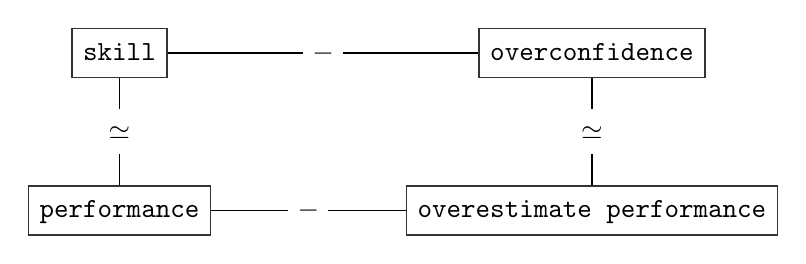
\begin{tikzpicture}
        [manifest/.style={rectangle,draw=black!80,semithick,minimum width=1cm,inner sep=4pt,text centered},
        latent/.style={circle,draw=black!80,thick,inner sep=2,text centered},
        latent_wide/.style={circle,draw=black!80,thick,inner sep=4,text centered},
        from/.style={<-,>=stealth',semithick},
        text height=1.75ex, text depth=.5ex]

\begin{scope}

% types
\node[manifest] at (0,0) (skill) {\texttt{skill}};

\node[manifest] at (6, 0) (overconfidence) {\texttt{overconfidence}};

\node[manifest] at (0, -2) (performance) {\texttt{performance}};

\node[manifest] at (6,-2) (estimate) {\texttt{overestimate performance}};


%arrows
\draw[-,>=stealth',semithick] (skill) -- node [fill=white] {$-$} (overconfidence);
\draw[-,>=stealth',semithick] (performance) -- node [fill=white] {$-$} (estimate);
\draw[-,>=stealth',semithick] (skill) -- node [fill=white] {$\simeq$} (performance);
\draw[-,>=stealth',semithick] (overconfidence) -- node [fill=white] {$\simeq$} (estimate);



\end{scope}

\end{tikzpicture}

  \end{center}
  %\caption{Subtypes of `AbstractSem`.}
  \label{fig:typetree}
\end{figure}

With $-$ signifying a negative association and $\simeq$ meaning measured by.



\begin{itemize}
 \item low skilled are more overconfident in assessing their skill than high skilled
\end{itemize}


\section{Mathematical Formulation}

\section{(Statistical) Models}

\subsection{Correction}
There are different ways to correct for the bias introduced by measurement error:
\begin{itemize}
 \item use different test performances to calculate skill and overconfidence, but a small test-retest correlation can bias the estimate towrds zero then (Krueger and Mueller, 2002)
\end{itemize}


\section{Open Questions / Ambiguities}


\end{document}
